\section{Results of evaluation}\label{sec:results-of-evaluation}

\subsection{Results of quantitative evaluation}\label{subsec:results-of-quantitative-evaluation}

This section presents (in tables~\ref{tab:4-1-section-a-results},~\ref{tab:4-1-section-b-results},~\ref{tab:4-1-section-c-results}, and~\ref{tab:4-1-section-d-results}) the results of the evaluation against the criteria for each area of GUI\@.
Table~\ref{tab:4-1-total-results} summarizes the results across all sections of evaluation.

\subsubsection{Architecture and structure}

The table~\ref{tab:4-1-section-a-results} presents the results of evaluation of criteria from section A\@.
\begin{itemize}
    \item varied support, depends on the goals
    \item some languages have more, some less
    \item Quid has little architectural support because it's a lightweight prototyping language
    \item surprisingly, some languages don't require the application concept \textendash\ in the end, it's only organizational
    \item low support for dialogs
    \item low support for third party components
\end{itemize}

\begin{longtblr}[
    caption = {Results of evaluation of section A},
    label = {tab:4-1-section-a-results},
]{
    colspec = {cccccccc},
    rowhead = 1,
    rows = {m},
}
    \hline[1pt]
    \rot{\textbf{No.}} & \rot{\textbf{\shortstack[l]{Gaouar \\ et al.}}}  & \rot{\textbf{\shortstack[l]{Khan\\ et al.}}} & \rot{\textbf{OpenUIDL}} & \rot{\textbf{Quid}} & \rot{\textbf{\shortstack[l]{Soude and\\ Koussonda}}} & \rot{\textbf{XANUI}} & \rot{\textbf{\shortstack[l]{Verhaeghe\\ et al.}}} \\
    \hline[1pt]
    \textbf{Total}     & 66,67\%                                          & 33,33\%                                      & 83,33\%                 & 16,67\%             & 33,33\%                                              & 66,67\%              & 50,00\%                                           \\
    \hline
    \textbf{A1}        & 100\% (\cmark)                                   & 0\% (\xmark)                                 & 100\% (\cmark)          & 0\% (\xmark)        & 0\% (\xmark)                                         & 100\% (\cmark)       & 100\% (\cmark)                                    \\
    \hline
    \textbf{A2}        & 100\% (\cmark)                                   & 100\% (\cmark)                               & 100\% (\cmark)          & 100\% (\cmark)      & 100\% (\cmark)                                       & 0\% (\xmark)         & 0\% (\xmark)                                      \\
    \hline
    \textbf{A3}        & 0\% (\xmark)                                     & 0\% (\xmark)                                 & 0\% (\xmark)            & 0\% (\xmark)        & 0\% (\xmark)                                         & 0\% (\xmark)         & 100\% (\cmark)                                    \\
    \hline
    \textbf{A4}        & 100\% (\cmark)                                   & 0\% (\xmark)                                 & 100\% (\cmark)          & 0\% (\xmark)        & 0\% (\xmark)                                         & 100\% (\cmark)       & 0\% (\xmark)                                      \\
    \hline
    \textbf{A5}        & 100\% (\cmark)                                   & 100\% (\cmark)                               & 100\% (\cmark)          & 0\% (\xmark)        & 100\% (\cmark)                                       & 100\% (\cmark)       & 100\% (\cmark)                                    \\
    \hline
    \textbf{A6}        & 0\% (\xmark)                                     & 0\% (\xmark)                                 & 100\% (\cmark)          & 0\% (\xmark)        & 0\% (\xmark)                                         & 100\% (\cmark)       & 0\% \xmark                                        \\
    \hline[1pt]
\end{longtblr}

\subsubsection{Logic and behavior}

Table~\ref{tab:4-1-section-b-results} presents the results of evaluation of criteria from section B\@.
\begin{itemize}
    \item general takeaway: varied, but in general low support for logic, though it also depends on the area
    \item most languages allow for handling events, but not too many allow for defining handlers
    \item support for predefined events is also varied
    \item similarly varied support for details of handlers - very little control structures (no iteration in handlers!)
    \item only XanUI has a mechanism for data validation
    \item a few languages can call external code; some even directly because they're annotation languages - they're embedded in an original language
    \item varied support for custom components, not always available; especially custom component methods were rare - only Quid did that
\end{itemize}
\begin{itemize}
    \item Khan explicitly states it doesnt support logic
    \item Verhaeghe isn't meant to directly describe applications, instead it's used for migrating; the metamodel is based on a AST so the new model doesnt introduce any meaningful concepts
    \item Gaouar has a metamodel, but it's rather rigid and it's unclear how logic and handlers would be modeled
    \item Quid allows for handling events and actually explicitly defining rudimentary handlers, but the language is limited in its capabilities
    \item OpenUIDL has good support for predefined events and custom components, but no support for handlers
    \item Soude and Koussonda supports handlers (at least for an input) and calling REST services; also has good support for expressions
    \item XanUI can do more because it's an annotation language that binds into whatever capabilities the language already has, but it still has some capabilities on its own
\end{itemize}

\begin{longtblr}[
    caption = {Results of evaluation of section B},
    label = {tab:4-1-section-b-results},
]{
    colspec = {cccccccc},
    rowhead = 1,
    rows = {m},
}
    \hline[1pt]
    \rot{\textbf{No.}} & \rot{\textbf{\shortstack[l]{Gaouar \\ et al.}}} & \rot{\textbf{\shortstack[l]{Khan\\ et al.}}} & \rot{\textbf{OpenUIDL}} & \rot{\textbf{Quid}} & \rot{\textbf{\shortstack[l]{Soude and\\ Koussonda}}} & \rot{\textbf{XANUI}} & \rot{\textbf{\shortstack[l]{Verhaeghe \\ et al.}}} \\
    \hline[1pt]
    \textbf{Total}     & 32,66\%                                         & 0,00\%                                       & 38,41\%                 & 30,63\%             & 51,56\%                                              & 66,30\%              & 19,17\%                                            \\
    \hline
    \textbf{B1}        & 100\% (\cmark)                                  & 0\% (\xmark)                                 & 100\% (\cmark)          & 100\% (\cmark)      & 100\% (\cmark)                                       & 100\% (\cmark)       & 100\% (\cmark)                                     \\
    \hline
    \textbf{B2}        & 17,50\%                                         & 0,00\%                                       & 82,50\%                 & 15,00\%             & 12,50\%                                              & 2,50\%               & 80,00\%                                            \\
    \hline[dashed]
    B2.1               & 20,00\%                                         & 0,00\%                                       & 30,00\%                 & 10,00\%             & 0,00\%                                               & 10,00\%              & 70,00\%                                            \\
    \textit{B2.1.1}    & \xmark                                          & \xmark                                       & \xmark                  & \xmark              & \xmark                                               & \xmark               & \cmark                                             \\
    \textit{B2.1.2}    & \xmark                                          & \xmark                                       & \xmark                  & \xmark              & \xmark                                               & \xmark               & \cmark                                             \\
    \textit{B2.1.3}    & \cmark                                          & \xmark                                       & \cmark                  & \cmark              & \xmark                                               & \cmark               & \cmark                                             \\
    \textit{B2.1.4}    & \xmark                                          & \xmark                                       & \xmark                  & \xmark              & \xmark                                               & \xmark               & \cmark                                             \\
    \textit{B2.1.5}    & \cmark                                          & \xmark                                       & \xmark                  & \xmark              & \xmark                                               & \xmark               & \xmark                                             \\
    \textit{B2.1.6}    & \xmark                                          & \xmark                                       & \cmark                  & \xmark              & \xmark                                               & \xmark               & \xmark                                             \\
    \textit{B2.1.7}    & \xmark                                          & \xmark                                       & \cmark                  & \xmark              & \xmark                                               & \xmark               & \cmark                                             \\
    \textit{B2.1.8}    & \xmark                                          & \xmark                                       & \xmark                  & \xmark              & \xmark                                               & \xmark               & \cmark                                             \\
    \textit{B2.1.9}    & \xmark                                          & \xmark                                       & \xmark                  & \xmark              & \xmark                                               & \xmark               & \xmark                                             \\
    \textit{B2.1.10}   & \xmark                                          & \xmark                                       & \xmark                  & \xmark              & \xmark                                               & \xmark               & \cmark                                             \\
    \hline[dashed]
    B2.2               & 0,00\%                                          & 0,00\%                                       & 100,00\%                & 0,00\%              & 0,00\%                                               & 0,00\%               & 100,00\%                                           \\
    \textit{B2.2.1}    & \xmark                                          & \xmark                                       & \cmark                  & \xmark              & \xmark                                               & \xmark               & \cmark                                             \\
    \textit{B2.2.2}    & \xmark                                          & \xmark                                       & \cmark                  & \xmark              & \xmark                                               & \xmark               & \cmark                                             \\
    \hline[dashed]
    B2.3               & 0,00\%                                          & 0,00\%                                       & 100,00\%                & 0,00\%              & 0,00\%                                               & 0,00\%               & 50,00\%                                            \\
    \textit{B2.3.1}    & \xmark                                          & \xmark                                       & \cmark                  & \xmark              & \xmark                                               & \xmark               & \cmark                                             \\
    \textit{B2.3.2}    & \xmark                                          & \xmark                                       & \cmark                  & \xmark              & \xmark                                               & \xmark               & \xmark                                             \\
    \hline[dashed]
    B2.4               & 50,00\%                                         & 0,00\%                                       & 100,00\%                & 50,00\%             & 50,00\%                                              & 0,00\%               & 100,00\%                                           \\
    \textit{B2.4.1}    & \xmark                                          & \xmark                                       & \cmark                  & \xmark              & \xmark                                               & \xmark               & \cmark                                             \\
    \textit{B2.4.2}    & \cmark                                          & \xmark                                       & \cmark                  & \cmark              & \cmark                                               & \xmark               & \cmark                                             \\
    \hline
    \textbf{B3}        & 100\% (\cmark)                                  & 0\% (\xmark)                                 & 0\% (\xmark)            & 100\% (\cmark)      & 100\% (\cmark)                                       & 100\% (\cmark)       & 0\% (\xmark)                                       \\
    \hline
    \textbf{B4}        & 30,00\%                                         & 0,00\%                                       & 0,00\%                  & 40,00\%             & 0,00\%                                               & 50,00\%              & 50,00\%                                            \\
    B4.1               & \cmark                                          & \xmark                                       & \xmark                  & \xmark              & \xmark                                               & \xmark               & \cmark                                             \\
    B4.2               & \xmark                                          & \xmark                                       & \xmark                  & \cmark              & \xmark                                               & \cmark               & \xmark                                             \\
    B4.3               & \cmark                                          & \xmark                                       & \xmark                  & \xmark              & \xmark                                               & \xmark               & \cmark                                             \\
    B4.4               & \xmark                                          & \xmark                                       & \xmark                  & \xmark              & \xmark                                               & \xmark               & \xmark                                             \\
    B4.5               & \xmark                                          & \xmark                                       & \xmark                  & \xmark              & \xmark                                               & \xmark               & \cmark                                             \\
    B4.6               & \xmark                                          & \xmark                                       & \xmark                  & \cmark              & \xmark                                               & \cmark               & \cmark                                             \\
    B4.7               & \cmark                                          & \xmark                                       & \xmark                  & \cmark              & \xmark                                               & \cmark               & \cmark                                             \\
    B4.8               & \xmark                                          & \xmark                                       & \xmark                  & \xmark              & \xmark                                               & \cmark               & \xmark                                             \\
    B4.9               & \xmark                                          & \xmark                                       & \xmark                  & \xmark              & \xmark                                               & \xmark               & \xmark                                             \\
    B4.10              & \xmark                                          & \xmark                                       & \xmark                  & \cmark              & \xmark                                               & \cmark               & \xmark                                             \\
    \hline
    \textbf{B5}        & 0,00\%                                          & 0,00\%                                       & 0,00\%                  & 0,00\%              & 0,00\%                                               & 100,00\%             & 0,00\%                                             \\
    B5.1               & \xmark                                          & \xmark                                       & \xmark                  & \xmark              & \xmark                                               & \cmark               & \xmark                                             \\
    B5.2               & \xmark                                          & \xmark                                       & \xmark                  & \xmark              & \xmark                                               & \cmark               & \xmark                                             \\
    B5.3               & \xmark                                          & \xmark                                       & \xmark                  & \xmark              & \xmark                                               & \cmark               & \xmark                                             \\
    B5.4               & \xmark                                          & \xmark                                       & \xmark                  & \xmark              & \xmark                                               & \cmark               & \xmark                                             \\
    B5.5               & \xmark                                          & \xmark                                       & \xmark                  & \xmark              & \xmark                                               & \cmark               & \xmark                                             \\
    B5.6               & \xmark                                          & \xmark                                       & \xmark                  & \xmark              & \xmark                                               & \cmark               & \xmark                                             \\
    \hline
    \textbf{B6}        & 100\% (\cmark)                                  & 0\% (\xmark)                                 & 0\% (\xmark)            & 0\% (\xmark)        & 100\% (\cmark)                                       & 100\% (\cmark)       & 0\% (\xmark)                                       \\
    \hline
    \textbf{B7}        & 0\% (\xmark)                                    & 0\% (\xmark)                                 & 0\% (\xmark)            & 0\% (\xmark)        & 0\% (\xmark)                                         & 100\% (\cmark)       & 0\% (\xmark)                                       \\
    \hline
    \textbf{B8}        & 0,00\%                                          & 0,00\%                                       & 50,00\%                 & 0,00\%              & 50,00\%                                              & 25,00\%              & 0,00\%                                             \\
    \hline[dashed]
    B8.1               & 0,00\%                                          & 0,00\%                                       & 0,00\%                  & 0,00\%              & 0,00\%                                               & 50,00\%              & 0,00\%                                             \\
    \textit{B8.1.1}    & \xmark                                          & \xmark                                       & \xmark                  & \xmark              & \xmark                                               & \cmark               & \xmark                                             \\
    \textit{B8.1.2}    & \xmark                                          & \xmark                                       & \xmark                  & \xmark              & \xmark                                               & \xmark               & \xmark                                             \\
    \hline[dashed]
    B8.2               & 0,00\%                                          & 0,00\%                                       & 100,00\%                & 0,00\%              & 100,00\%                                             & 0,00\%               & 0,00\%                                             \\
    \textit{B8.2.1}    & \xmark                                          & \xmark                                       & \cmark                  & \xmark              & \cmark                                               & \xmark               & \xmark                                             \\
    \textit{B8.2.2}    & \xmark                                          & \xmark                                       & \cmark                  & \xmark              & \cmark                                               & \xmark               & \xmark                                             \\
    \hline
    \textbf{B9}        & 0\% (\xmark)                                    & 0\% (\xmark)                                 & 100\% (\cmark)          & 0\% (\xmark)        & 100\% (\cmark)                                       & 100\% (\cmark)       & 0\% (\xmark)                                       \\
    \hline
    \textbf{B10}       & 44,44\%                                         & 0,00\%                                       & 55,56\%                 & 33,33\%             & 66,67\%                                              & 55,56\%              & 0,00\%                                             \\
    B10.1              & \cmark                                          & \xmark                                       & \cmark                  & \cmark              & \cmark                                               & \cmark               & \xmark                                             \\
    B10.2              & \cmark                                          & \xmark                                       & \cmark                  & \cmark              & \cmark                                               & \cmark               & \xmark                                             \\
    B10.3              & \xmark                                          & \xmark                                       & \cmark                  & \xmark              & \cmark                                               & \cmark               & \xmark                                             \\
    B10.4              & \xmark                                          & \xmark                                       & \xmark                  & \xmark              & \xmark                                               & \xmark               & \xmark                                             \\
    B10.5              & \cmark                                          & \xmark                                       & \cmark                  & \cmark              & \cmark                                               & \cmark               & \xmark                                             \\
    B10.6              & \xmark                                          & \xmark                                       & \xmark                  & \xmark              & \xmark                                               & \xmark               & \xmark                                             \\
    B10.7              & \cmark                                          & \xmark                                       & \cmark                  & \xmark              & \cmark                                               & \xmark               & \xmark                                             \\
    B10.8              & \xmark                                          & \xmark                                       & \xmark                  & \xmark              & \xmark                                               & \xmark               & \xmark                                             \\
    B10.9              & \xmark                                          & \xmark                                       & \xmark                  & \xmark              & \cmark                                               & \cmark               & \xmark                                             \\
    \hline
    \textbf{B11}       & 0,00\%                                          & 0,00\%                                       & 6,25\%                  & 12,50\%             & 72,92\%                                              & 12,50\%              & 0,00\%                                             \\
    \hline[dashed]
    B11.1              & 0,00\%                                          & 0,00\%                                       & 25,00\%                 & 0,00\%              & 91,67\%                                              & 0,00\%               & 0,00\%                                             \\
    \textit{B11.1.1}   & \xmark                                          & \xmark                                       & \cmark                  & \xmark              & \cmark                                               & \xmark               & \xmark                                             \\
    \textit{B11.1.2}   & \xmark                                          & \xmark                                       & \cmark                  & \xmark              & \cmark                                               & \xmark               & \xmark                                             \\
    \textit{B11.1.3}   & \xmark                                          & \xmark                                       & \xmark                  & \xmark              & \cmark                                               & \xmark               & \xmark                                             \\
    \textit{B11.1.4}   & \xmark                                          & \xmark                                       & \xmark                  & \xmark              & \cmark                                               & \xmark               & \xmark                                             \\
    \textit{B11.1.5}   & \xmark                                          & \xmark                                       & \xmark                  & \xmark              & \cmark                                               & \xmark               & \xmark                                             \\
    \textit{B11.1.6}   & \xmark                                          & \xmark                                       & \xmark                  & \xmark              & \xmark                                               & \xmark               & \xmark                                             \\
    \textit{B11.1.7}   & \xmark                                          & \xmark                                       & \cmark                  & \xmark              & \cmark                                               & \xmark               & \xmark                                             \\
    \textit{B11.1.8}   & \xmark                                          & \xmark                                       & \xmark                  & \xmark              & \cmark                                               & \xmark               & \xmark                                             \\
    \textit{B11.1.9}   & \xmark                                          & \xmark                                       & \xmark                  & \xmark              & \cmark                                               & \xmark               & \xmark                                             \\
    \textit{B11.1.10}  & \xmark                                          & \xmark                                       & \xmark                  & \xmark              & \cmark                                               & \xmark               & \xmark                                             \\
    \textit{B11.1.11}  & \xmark                                          & \xmark                                       & \xmark                  & \xmark              & \cmark                                               & \xmark               & \xmark                                             \\
    \textit{B11.1.12}  & \xmark                                          & \xmark                                       & \xmark                  & \xmark              & \cmark                                               & \xmark               & \xmark                                             \\
    \hline[dashed]
    B11.2              & 0,00\%                                          & 0,00\%                                       & 0,00\%                  & 0,00\%              & 0,00\%                                               & 0,00\%               & 0,00\%                                             \\
    \textit{B11.2.1}   & \xmark                                          & \xmark                                       & \xmark                  & \xmark              & \xmark                                               & \xmark               & \xmark                                             \\
    \textit{B11.2.2}   & \xmark                                          & \xmark                                       & \xmark                  & \xmark              & \xmark                                               & \xmark               & \xmark                                             \\
    \textit{B11.2.3}   & \xmark                                          & \xmark                                       & \xmark                  & \xmark              & \xmark                                               & \xmark               & \xmark                                             \\
    \hline[dashed]
    B11.3              & 0,00\%                                          & 0,00\%                                       & 0,00\%                  & 50,00\%             & 100,00\%                                             & 50,00\%              & 0,00\%                                             \\
    \textit{B11.3.1}   & \xmark                                          & \xmark                                       & \xmark                  & \xmark              & \cmark                                               & \xmark               & \xmark                                             \\
    \textit{B11.3.2}   & \xmark                                          & \xmark                                       & \xmark                  & \cmark              & \cmark                                               & \cmark               & \xmark                                             \\
    \hline[dashed]
    B11.4              & \xmark                                          & \xmark                                       & \xmark                  & \xmark              & \cmark                                               & \xmark               & \xmark                                             \\
    \hline
    \textbf{B12}       & 0,00\%                                          & 0,00\%                                       & 66,67\%                 & 66,67\%             & 16,67\%                                              & 50,00\%              & 0,00\%                                             \\
    B12.1              & \xmark                                          & \xmark                                       & \cmark                  & \cmark              & \cmark                                               & \cmark               & \xmark                                             \\
    B12.2              & \xmark                                          & \xmark                                       & \cmark                  & \xmark              & \xmark                                               & \cmark               & \xmark                                             \\
    B12.3              & \xmark                                          & \xmark                                       & \cmark                  & \xmark              & \xmark                                               & \xmark               & \xmark                                             \\
    B12.4              & \xmark                                          & \xmark                                       & \xmark                  & \cmark              & \xmark                                               & \cmark               & \xmark                                             \\
    B12.5              & \xmark                                          & \xmark                                       & \xmark                  & \cmark              & \xmark                                               & \xmark               & \xmark                                             \\
    B12.6              & \xmark                                          & \xmark                                       & \cmark                  & \cmark              & \xmark                                               & \xmark               & \xmark                                             \\
    \hline[1pt]
\end{longtblr}

\subsubsection{Component support}

The table~\ref{tab:4-1-section-c-results} presents the results of evaluation of criteria for section C\@.
\begin{itemize}
    \item general takeaway: low to medium support
    \item the lowest support for complex output components - few representation have thought about providing anything more complex
    \item specialized containers are also rather poorly supported
    \item best support for interaction components and simple outputs, though still not remarkable (around 50\%)
    \item inputs quite well supported, though not always can be well customized
\end{itemize}
\begin{itemize}
    \item Quid again doesn't have too much stuff, the language is simple and minimal
    \item Gaouar and XanUI dont support too many concepts either; the former just doesn't have many components in the model; the latter might not need that many because it bases on the original implementation language
    \item anything else is just a matter of a more or less detailed model
\end{itemize}

\begin{longtblr}[
    caption = {Results of evaluation of section C},
    label = {tab:4-1-section-c-results},
]{
    colspec = {cccccccc},
    rowhead = 1,
    rows = {m},
}
    \hline[1pt]
    \rot{\textbf{No.}} & \rot{\textbf{\shortstack[l]{Gaouar\\ et al.}}} & \rot{\textbf{\shortstack[l]{Khan\\ et al.}}} & \rot{\textbf{OpenUIDL}} & \rot{\textbf{Quid}} & \rot{\textbf{\shortstack[l]{Soude and\\ Koussonda}}} & \rot{\textbf{XANUI}} & \rot{\textbf{\shortstack[l]{Verhaeghe\\ et al.}}} \\
    \hline[1pt]
    \textbf{Total}     & 17,93\%                                        & 36,30\%                                      & 45,82\%                 & 13,20\%             & 49,10\%                                              & 28,66\%              & 55,37\%                                           \\
    \hline
    \textbf{C1}        & 0,00\%                                         & 50,00\%                                      & 33,33\%                 & 33,33\%             & 50,00\%                                              & 16,67\%              & 50,00\%                                           \\
    C1.1               & \xmark                                         & \cmark                                       & \xmark                  & \cmark              & \xmark                                               & \xmark               & \cmark                                            \\
    C1.2               & \xmark                                         & \xmark                                       & \cmark                  & \xmark              & \xmark                                               & \xmark               & \xmark                                            \\
    C1.3               & \xmark                                         & \cmark                                       & \xmark                  & \cmark              & \cmark                                               & \xmark               & \xmark                                            \\
    C1.4               & \xmark                                         & \xmark                                       & \xmark                  & \xmark              & \cmark                                               & \cmark               & \cmark                                            \\
    C1.5               & \xmark                                         & \cmark                                       & \xmark                  & \xmark              & \xmark                                               & \xmark               & \xmark                                            \\
    C1.6               & \xmark                                         & \xmark                                       & \cmark                  & \xmark              & \cmark                                               & \xmark               & \cmark                                            \\
    \hline
    \textbf{C2}        & 50,00\%                                        & 37,50\%                                      & 50,00\%                 & 25,00\%             & 50,00\%                                              & 37,50\%              & 62,50\%                                           \\
    C2.1               & \cmark                                         & \cmark                                       & \cmark                  & \xmark              & \cmark                                               & \cmark               & \cmark                                            \\
    C2.2               & \xmark                                         & \xmark                                       & \cmark                  & \xmark              & \xmark                                               & \xmark               & \cmark                                            \\
    C2.3               & \xmark                                         & \xmark                                       & \xmark                  & \xmark              & \xmark                                               & \xmark               & \xmark                                            \\
    C2.4               & \cmark                                         & \cmark                                       & \cmark                  & \cmark              & \cmark                                               & \cmark               & \cmark                                            \\
    C2.5               & \xmark                                         & \xmark                                       & \xmark                  & \xmark              & \xmark                                               & \xmark               & \xmark                                            \\
    C2.6               & \cmark                                         & \cmark                                       & \cmark                  & \xmark              & \cmark                                               & \cmark               & \cmark                                            \\
    C2.7               & \xmark                                         & \xmark                                       & \xmark                  & \cmark              & \cmark                                               & \xmark               & \cmark                                            \\
    C2.8               & \cmark                                         & \xmark                                       & \xmark                  & \xmark              & \xmark                                               & \xmark               & \xmark                                            \\
    \hline
    \textbf{C3}        & 0,00\%                                         & 0,00\%                                       & 0,00\%                  & 0,00\%              & 100,00\%                                             & 0,00\%               & 50,00\%                                           \\
    C3.1               & \xmark                                         & \xmark                                       & \xmark                  & \xmark              & \cmark                                               & \xmark               & \cmark                                            \\
    C3.2               & \xmark                                         & \xmark                                       & \xmark                  & \xmark              & \cmark                                               & \xmark               & \xmark                                            \\
    \hline
    \textbf{C4}        & 42,31\%                                        & 50,96\%                                      & 72,12\%                 & 0,96\%              & 55,77\%                                              & 50,00\%              & 61,54\%                                           \\
    C4.1               & \xmark                                         & \xmark                                       & \cmark                  & \xmark              & \cmark                                               & \xmark               & \xmark                                            \\
    C4.2               & \xmark                                         & \cmark                                       & \xmark                  & \xmark              & \xmark                                               & \xmark               & \xmark                                            \\
    \hline[dashed]
    C4.3               & 38,46\%                                        & 7,69\%                                       & 76,92\%                 & 7,69\%              & 46,15\%                                              & 0,00\%               & 92,31\%                                           \\
    \textit{C4.3.1}    & \cmark                                         & \xmark                                       & \cmark                  & \xmark              & \cmark                                               & \xmark               & \cmark                                            \\
    \textit{C4.3.2}    & \xmark                                         & \xmark                                       & \cmark                  & \xmark              & \xmark                                               & \xmark               & \cmark                                            \\
    \textit{C4.3.3}    & \xmark                                         & \xmark                                       & \cmark                  & \xmark              & \cmark                                               & \xmark               & \cmark                                            \\
    \textit{C4.3.4}    & \xmark                                         & \xmark                                       & \cmark                  & \xmark              & \xmark                                               & \xmark               & \cmark                                            \\
    \textit{C4.3.5}    & \xmark                                         & \xmark                                       & \xmark                  & \xmark              & \xmark                                               & \xmark               & \cmark                                            \\
    \textit{C4.3.6}    & \cmark                                         & \xmark                                       & \cmark                  & \xmark              & \cmark                                               & \xmark               & \cmark                                            \\
    \textit{C4.3.7}    & \xmark                                         & \xmark                                       & \cmark                  & \xmark              & \cmark                                               & \xmark               & \cmark                                            \\
    \textit{C4.3.8}    & \cmark                                         & \xmark                                       & \cmark                  & \xmark              & \cmark                                               & \xmark               & \cmark                                            \\
    \textit{C4.3.8}    & \xmark                                         & \xmark                                       & \xmark                  & \xmark              & \xmark                                               & \xmark               & \cmark                                            \\
    \textit{C4.3.9}    & \xmark                                         & \xmark                                       & \xmark                  & \xmark              & \xmark                                               & \xmark               & \cmark                                            \\
    \textit{C4.3.10}   & \xmark                                         & \xmark                                       & \cmark                  & \xmark              & \xmark                                               & \xmark               & \xmark                                            \\
    \textit{C4.3.11}   & \cmark                                         & \cmark                                       & \cmark                  & \cmark              & \cmark                                               & \xmark               & \cmark                                            \\
    \textit{C4.3.12}   & \cmark                                         & \xmark                                       & \cmark                  & \xmark              & \xmark                                               & \xmark               & \cmark                                            \\
    \hline[dashed]
    C4.4               & \cmark                                         & \cmark                                       & \cmark                  & \xmark              & \cmark                                               & \cmark               & \cmark                                            \\
    C4.5               & \xmark                                         & \cmark                                       & \cmark                  & \xmark              & \cmark                                               & \cmark               & \cmark                                            \\
    C4.6               & \cmark                                         & \cmark                                       & \xmark                  & \xmark              & \xmark                                               & \xmark               & \xmark                                            \\
    C4.7               & \cmark                                         & \xmark                                       & \cmark                  & \xmark              & \cmark                                               & \cmark               & \cmark                                            \\
    C4.8               & \xmark                                         & \xmark                                       & \cmark                  & \xmark              & \xmark                                               & \cmark               & \cmark                                            \\
    \hline
    \textbf{C5}        & 0,00\%                                         & 25,00\%                                      & 87,50\%                 & 0,00\%              & 25,00\%                                              & 33,33\%              & 75,00\%                                           \\
    \hline[dashed]
    C5.1               & 0,00\%                                         & 0,00\%                                       & 75,00\%                 & 0,00\%              & 0,00\%                                               & 66,67\%              & 50,00\%                                           \\
    \textit{C5.1.1}    & \xmark                                         & \xmark                                       & \xmark                  & \xmark              & \xmark                                               & \cmark               & \xmark                                            \\
    \textit{C5.1.2}    & \xmark                                         & \xmark                                       & \cmark                  & \xmark              & \xmark                                               & \cmark               & \cmark                                            \\
    \textit{C5.1.3}    & \xmark                                         & \xmark                                       & 0.5                     & \xmark              & \xmark                                               & \xmark               & \cmark                                            \\
    \textit{C5.1.4}    & \xmark                                         & \xmark                                       & 0.5                     & \xmark              & \xmark                                               & \xmark               & \xmark                                            \\
    \textit{C5.1.5}    & \xmark                                         & \xmark                                       & \cmark                  & \xmark              & \xmark                                               & \cmark               & \cmark                                            \\
    \textit{C5.1.6}    & \xmark                                         & \xmark                                       & \cmark                  & \xmark              & \xmark                                               & \cmark               & \xmark                                            \\
    \hline[dashed]
    C5.2               & 0,00\%                                         & 50,00\%                                      & 100,00\%                & 0,00\%              & 50,00\%                                              & 0,00\%               & 100,00\%                                          \\
    \textit{C5.2.1}    & \xmark                                         & \xmark                                       & \cmark                  & \xmark              & \xmark                                               & \xmark               & \cmark                                            \\
    \textit{C5.2.2}    & \xmark                                         & \cmark                                       & \cmark                  & \xmark              & \cmark                                               & \xmark               & \cmark                                            \\
    \hline
    \textbf{C6}        & 33,33\%                                        & 100,00\%                                     & 66,67\%                 & 33,33\%             & 33,33\%                                              & 66,67\%              & 66,67\%                                           \\
    C6.1               & \cmark                                         & \cmark                                       & \cmark                  & \cmark              & \cmark                                               & \cmark               & \cmark                                            \\
    C6.2               & \xmark                                         & \cmark                                       & \cmark                  & \xmark              & \xmark                                               & \cmark               & \cmark                                            \\
    C6.3               & \xmark                                         & \cmark                                       & \xmark                  & \xmark              & \xmark                                               & \xmark               & \xmark                                            \\
    \hline[1pt]
\end{longtblr}

\subsubsection{Appearance}

The table~\ref{tab:4-1-section-d-results} presents the results of evaluation of criteria for section D\@.
\begin{itemize}
    \item extremely varied support - some languages don't allow any styling and some are very flexible
    \item most languages support a linear layout, some specify an additional one; though other layouts are not that necessary, the linear layout is enough most of the time
    \item support for media queries is relatively high \textendash\ 3 out of 7 languages
    \item varied support for sizing and positioning - some languages provide most or all methods, some none
    \item little support for sizing units, only OpenUIDL implements a lot
    \item other styling is either included or not in general
    \item two representations allow for using CSS
\end{itemize}
\begin{itemize}
    \item Quid and Soude practically dismiss the issue of appearance
    \item XanUI also doesn't concern itself with appearance, as this problem might be resolved natively
    \item Verhaeghe, Gaouar and Khan just have a more or less detailed model
    \item OpenUIDL is very expressive - actually scores 100\% almost everywhere, with the exception of layouts (it's mostly targeted towards Web development, so layouts other than linear and flex aren't necessary)
\end{itemize}

\begin{longtblr}[
    caption = {Results of evaluation of section D},
    label = {tab:4-1-section-d-results},
]{
    colspec = {cccccccc},
    rowhead = 1,
    rows = {m},
}
    \hline[1pt]
    \rot{\textbf{No.}} & \rot{\textbf{\shortstack[l]{Gaouar\\ et al.}}} & \rot{\textbf{\shortstack[l]{Khan\\ et al.}}} & \rot{\textbf{OpenUIDL}} & \rot{\textbf{Quid}} & \rot{\textbf{\shortstack[l]{Soude and\\ Koussonda}}} & \rot{\textbf{XANUI}} & \rot{\textbf{\shortstack[l]{Verhaeghe\\ et al.}}} \\
    \hline[1pt]
    \textbf{Total}     & 40,42\%                                        & 68,65\%                                      & 89,38\%                 & 2,50\%              & 0,00\%                                               & 5,00\%               & 28,33\%                                           \\
    \hline
    \textbf{D1}        & 40,00\%                                        & 20,00\%                                      & 40,00\%                 & 20,00\%             & 0,00\%                                               & 40,00\%              & 60,00\%                                           \\
    D1.1               & \cmark                                         & \cmark                                       & \cmark                  & \cmark              & \xmark                                               & \cmark               & \cmark                                            \\
    D1.2               & \xmark                                         & \xmark                                       & \cmark                  & \xmark              & \xmark                                               & \xmark               & \xmark                                            \\
    D1.3               & \xmark                                         & \xmark                                       & \xmark                  & \xmark              & \xmark                                               & \xmark               & \cmark                                            \\
    D1.4               & \cmark                                         & \xmark                                       & \xmark                  & \xmark              & \xmark                                               & \xmark               & \xmark                                            \\
    D1.5               & \xmark                                         & \xmark                                       & \xmark                  & \xmark              & \xmark                                               & \cmark               & \cmark                                            \\
    \hline
    \textbf{D2}        & 100\% (\cmark)                                 & 100\% (\cmark)                               & 100\% (\cmark)          & 0\% (\xmark)        & 0\% (\xmark)                                         & 0\% (\xmark)         & 0\% (\xmark)                                      \\
    \hline
    \textbf{D3}        & 33,33\%                                        & 100,00\%                                     & 100,00\%                & 0,00\%              & 0,00\%                                               & 0,00\%               & 66,67\%                                           \\
    D3.1               & \xmark                                         & \cmark                                       & \cmark                  & \xmark              & \xmark                                               & \xmark               & \cmark                                            \\
    D3.2               & \cmark                                         & \cmark                                       & \cmark                  & \xmark              & \xmark                                               & \xmark               & \cmark                                            \\
    D3.3               & \xmark                                         & \cmark                                       & \cmark                  & \xmark              & \xmark                                               & \xmark               & \xmark                                            \\
    \hline
    \textbf{D4}        & 25,00\%                                        & 12,50\%                                      & 75,00\%                 & 0,00\%              & 0,00\%                                               & 0,00\%               & 25,00\%                                           \\
    D4.1               & \cmark                                         & \xmark                                       & \cmark                  & \xmark              & \xmark                                               & \xmark               & \cmark                                            \\
    D4.2               & \xmark                                         & \cmark                                       & \xmark                  & \xmark              & \xmark                                               & \xmark               & \xmark                                            \\
    D4.3               & \xmark                                         & \xmark                                       & \xmark                  & \xmark              & \xmark                                               & \xmark               & \xmark                                            \\
    D4.4               & \cmark                                         & \xmark                                       & \cmark                  & \xmark              & \xmark                                               & \xmark               & \cmark                                            \\
    D4.5               & \xmark                                         & \xmark                                       & \cmark                  & \xmark              & \xmark                                               & \xmark               & \xmark                                            \\
    D4.6               & \xmark                                         & \xmark                                       & \cmark                  & \xmark              & \xmark                                               & \xmark               & \xmark                                            \\
    D4.7               & \xmark                                         & \xmark                                       & \cmark                  & \xmark              & \xmark                                               & \xmark               & \xmark                                            \\
    D4.8               & \xmark                                         & \xmark                                       & \cmark                  & \xmark              & \xmark                                               & \xmark               & \xmark                                            \\
    \hline
    \textbf{D5}        & 25,00\%                                        & 75,00\%                                      & 100,00\%                & 0,00\%              & 0,00\%                                               & 0,00\%               & 75,00\%                                           \\
    D5.1               & \cmark                                         & \cmark                                       & \cmark                  & \xmark              & \xmark                                               & \xmark               & \cmark                                            \\
    D5.2               & \xmark                                         & \cmark                                       & \cmark                  & \xmark              & \xmark                                               & \xmark               & \cmark                                            \\
    D5.3               & \xmark                                         & \cmark                                       & \cmark                  & \xmark              & \xmark                                               & \xmark               & \cmark                                            \\
    D5.4               & \xmark                                         & \xmark                                       & \cmark                  & \xmark              & \xmark                                               & \xmark               & \xmark                                            \\
    \hline
    \textbf{D6}        & 16,67\%                                        & 58,33\%                                      & 100,00\%                & 0,00\%              & 0,00\%                                               & 0,00\%               & 0,00\%                                            \\
    D6.1               & \cmark                                         & \cmark                                       & \cmark                  & \xmark              & \xmark                                               & \xmark               & \xmark                                            \\
    D6.2               & \cmark                                         & \cmark                                       & \cmark                  & \xmark              & \xmark                                               & \xmark               & \xmark                                            \\
    D6.3               & \xmark                                         & \cmark                                       & \cmark                  & \xmark              & \xmark                                               & \xmark               & \xmark                                            \\
    D6.4               & \xmark                                         & \xmark                                       & \cmark                  & \xmark              & \xmark                                               & \xmark               & \xmark                                            \\
    D6.5               & \xmark                                         & \cmark                                       & \cmark                  & \xmark              & \xmark                                               & \xmark               & \xmark                                            \\
    D6.7               & \xmark                                         & \cmark                                       & \cmark                  & \xmark              & \xmark                                               & \xmark               & \xmark                                            \\
    D6.8               & \xmark                                         & \cmark                                       & \cmark                  & \xmark              & \xmark                                               & \xmark               & \xmark                                            \\
    D6.9               & \xmark                                         & \xmark                                       & \cmark                  & \xmark              & \xmark                                               & \xmark               & \xmark                                            \\
    D6.10              & \xmark                                         & \xmark                                       & \cmark                  & \xmark              & \xmark                                               & \xmark               & \xmark                                            \\
    D6.11              & \xmark                                         & \cmark                                       & \cmark                  & \xmark              & \xmark                                               & \xmark               & \xmark                                            \\
    D6.12              & \xmark                                         & \xmark                                       & \cmark                  & \xmark              & \xmark                                               & \xmark               & \xmark                                            \\
    D6.13              & \xmark                                         & \xmark                                       & \cmark                  & \xmark              & \xmark                                               & \xmark               & \xmark                                            \\
    \hline
    \textbf{D7}        & 83,33\%                                        & 83,33\%                                      & 100,00\%                & 0,00\%              & 0,00\%                                               & 0,00\%               & 0,00\%                                            \\
    D7.1               & \cmark                                         & \cmark                                       & \cmark                  & \xmark              & \xmark                                               & \xmark               & \xmark                                            \\
    D7.2               & \cmark                                         & \cmark                                       & \cmark                  & \xmark              & \xmark                                               & \xmark               & \xmark                                            \\
    D7.3               & \xmark                                         & \xmark                                       & \cmark                  & \xmark              & \xmark                                               & \xmark               & \xmark                                            \\
    D7.4               & \cmark                                         & \cmark                                       & \cmark                  & \xmark              & \xmark                                               & \xmark               & \xmark                                            \\
    D7.5               & \cmark                                         & \cmark                                       & \cmark                  & \xmark              & \xmark                                               & \xmark               & \xmark                                            \\
    D7.6               & \cmark                                         & \cmark                                       & \cmark                  & \xmark              & \xmark                                               & \xmark               & \xmark                                            \\
    \hline
    \textbf{D8}        & 0\% (\xmark)                                   & 100\% (\cmark)                               & 100\% (\cmark)          & 0\% (\xmark)        & 0\% (\xmark)                                         & 0\% (\xmark)         & 0\% (\xmark)                                      \\
    \hline[1pt]
\end{longtblr}

\subsubsection{Summary}

Table~\ref{tab:4-1-total-results} and figures~\ref{fig:4-1-results-per-section},~\ref{fig:4-1-results-per-representation}, and~\ref{fig:4-1-results-total} present the total results.
My conclusions are:
\begin{itemize}
    \item some languages have good support in some areas, but no language includes everything
    \item none of the languages seem really flexible and productive
    \item Quid is a very simple language, simple support for logic, but no appearance and components
    \item Soude and Koussonda, Khan have some strong and weak areas
    \item XanUI has strong support for logic, but little components and support for appearance \textendash\ however, this might be because it doesn't need to be handled by the language
    \item Verhaeghe and Gaouar have a little bit of everything, but do not excel in any particular area
    \item OpenUIDL is the most expressive, with good architectural support, decent component support and strong customizability of appearance; the only weak area is logic - there aren't many possibilities to define handlers and state and change it
\end{itemize}

\begin{longtblr}[
    caption = {Summary of results of evaluation represenations},
    label = {tab:4-1-total-results},
]{
    colspec = {cccccccc},
    rowhead = 1,
    rows = {m},
}
    \hline[1pt]
    \rot{\textbf{Section}} & \rot{\textbf{\shortstack[l]{Gaouar\\ et al.}}} & \rot{\textbf{\shortstack[l]{Khan\\ et al.}}} & \rot{\textbf{OpenUIDL}} & \rot{\textbf{Quid}} & \rot{\textbf{\shortstack[l]{Soude and\\ Koussonda}}} & \rot{\textbf{XANUI}} & \rot{\textbf{\shortstack[l]{Verhaeghe\\ et al.}}} \\
    \hline[1pt]
    \textbf{Total}         & 40,17\%                                        & 36,47\%                                      & 65,68\%                 & 16,31\%             & 34,31\%                                              & 43,00\%              & 39,61\%                                           \\
    \textbf{A}             & 66,67\%                                        & 33,33\%                                      & 83,33\%                 & 16,67\%             & 33,33\%                                              & 66,67\%              & 50,00\%                                           \\
    \textbf{B}             & 32,66\%                                        & 0,00\%                                       & 38,41\%                 & 30,63\%             & 51,56\%                                              & 66,30\%              & 19,17\%                                           \\
    \textbf{C}             & 20,94\%                                        & 43,91\%                                      & 51,60\%                 & 15,44\%             & 52,35\%                                              & 34,03\%              & 60,95\%                                           \\
    \textbf{D}             & 40,42\%                                        & 68,65\%                                      & 89,38\%                 & 2,50\%              & 0,00\%                                               & 5,00\%               & 28,33\%                                           \\
    \hline[1pt]
\end{longtblr}

\begin{figure}
    \centering
    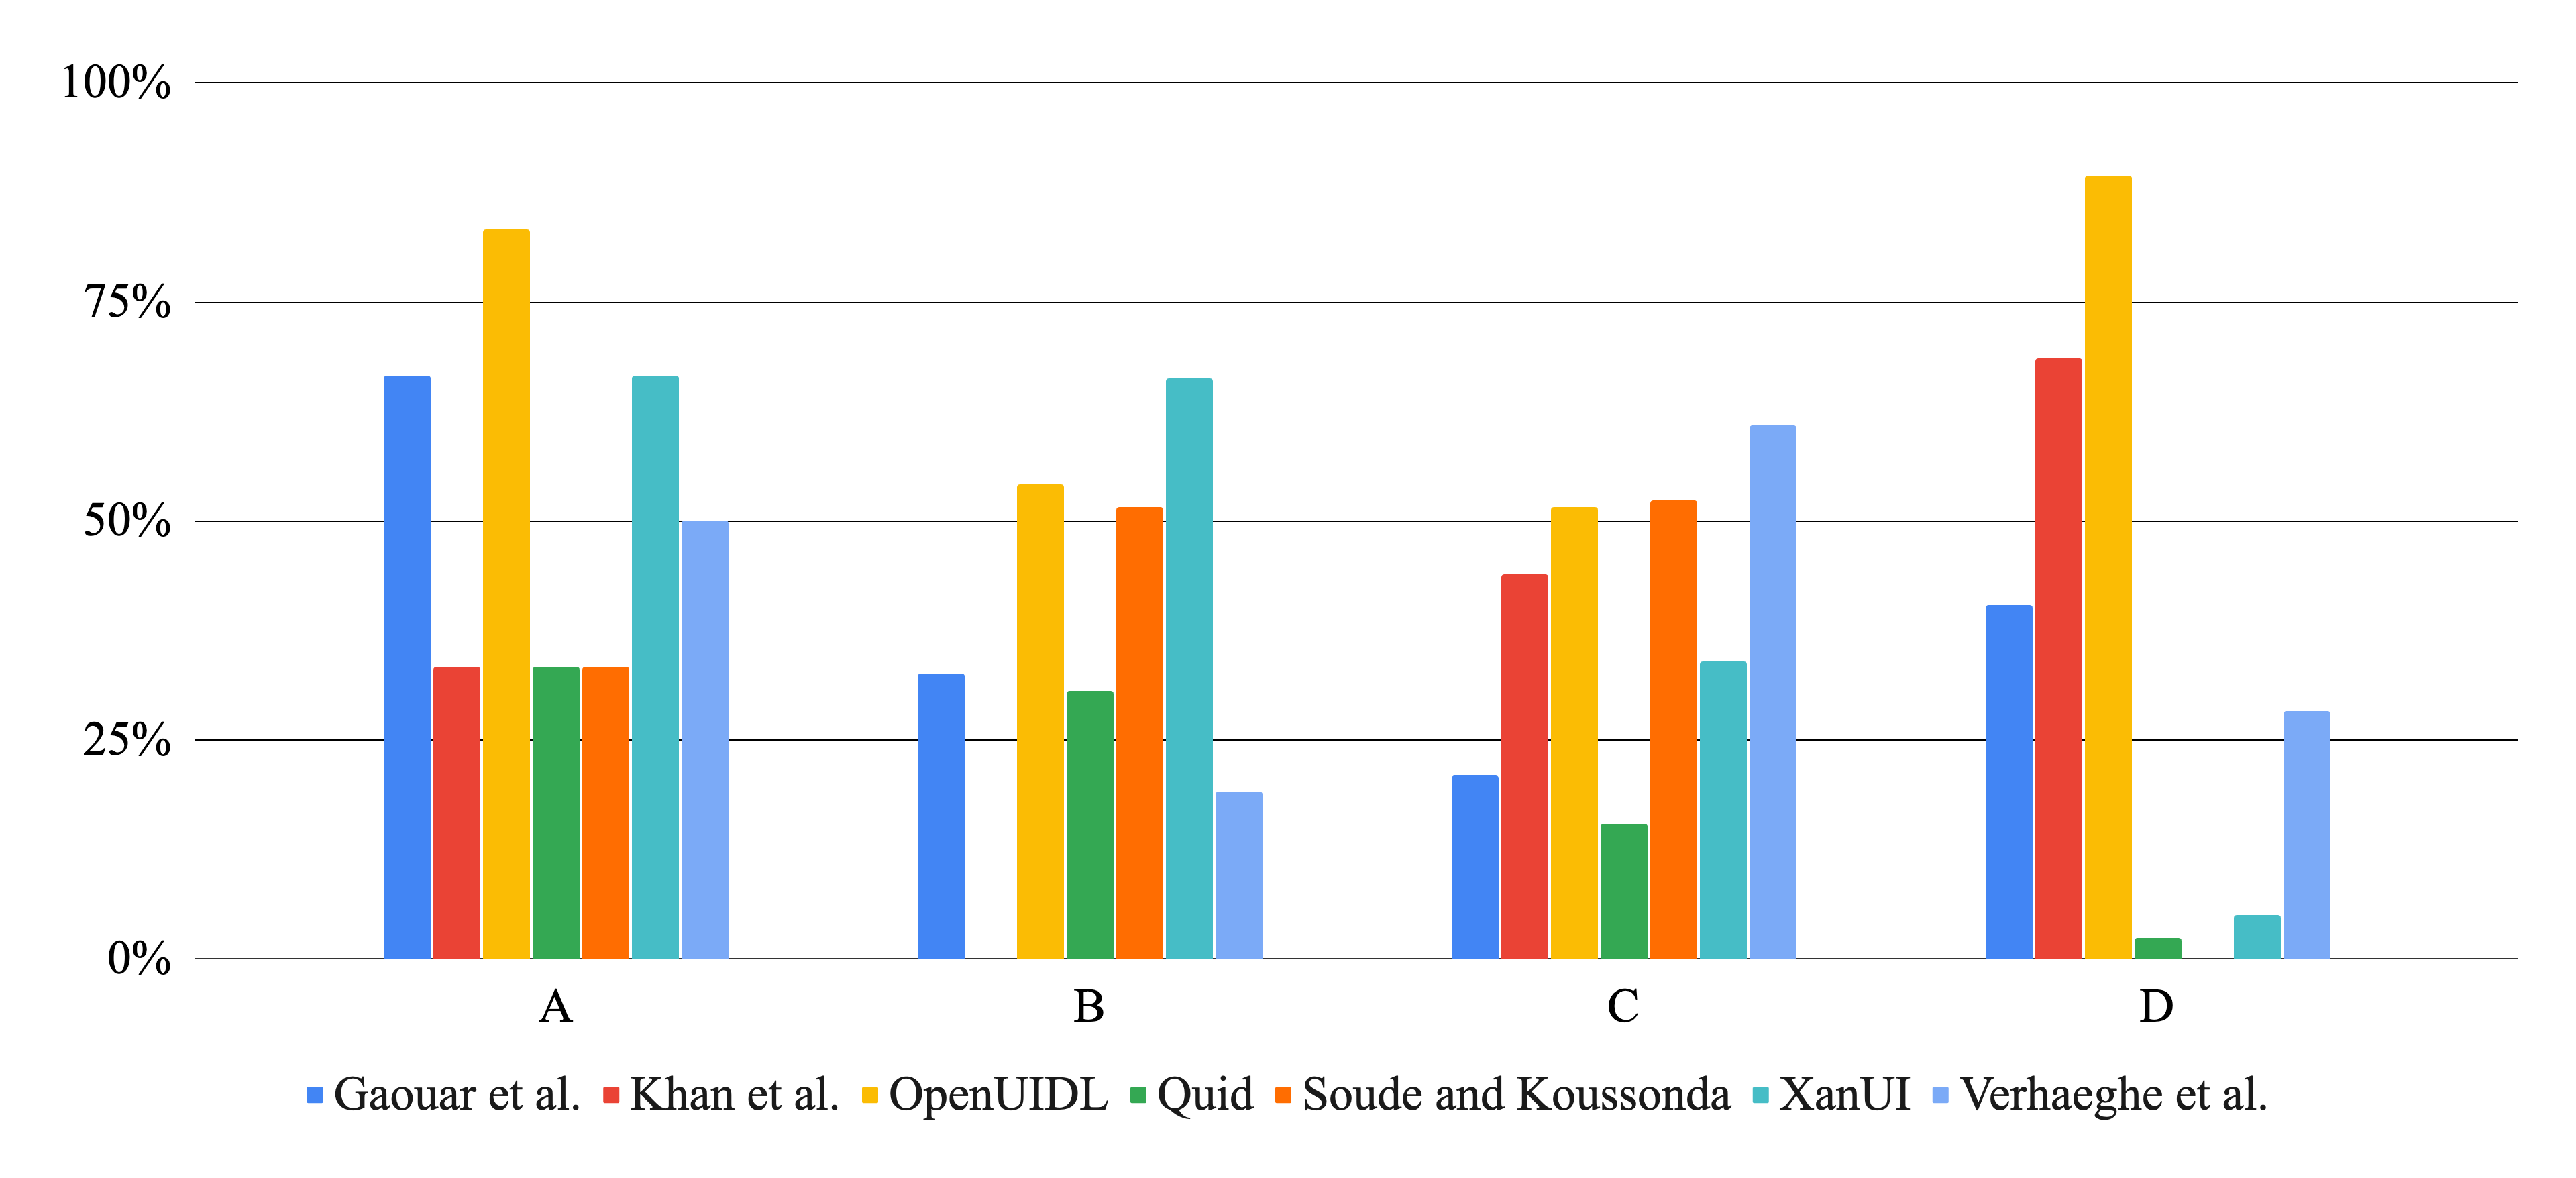
\includegraphics[width=\textwidth]{4-results-and-discussion/results-per-section}
    \caption{Results of the evaluation, presented per section}
    \label{fig:4-1-results-per-section}
\end{figure}

\begin{figure}
    \centering
    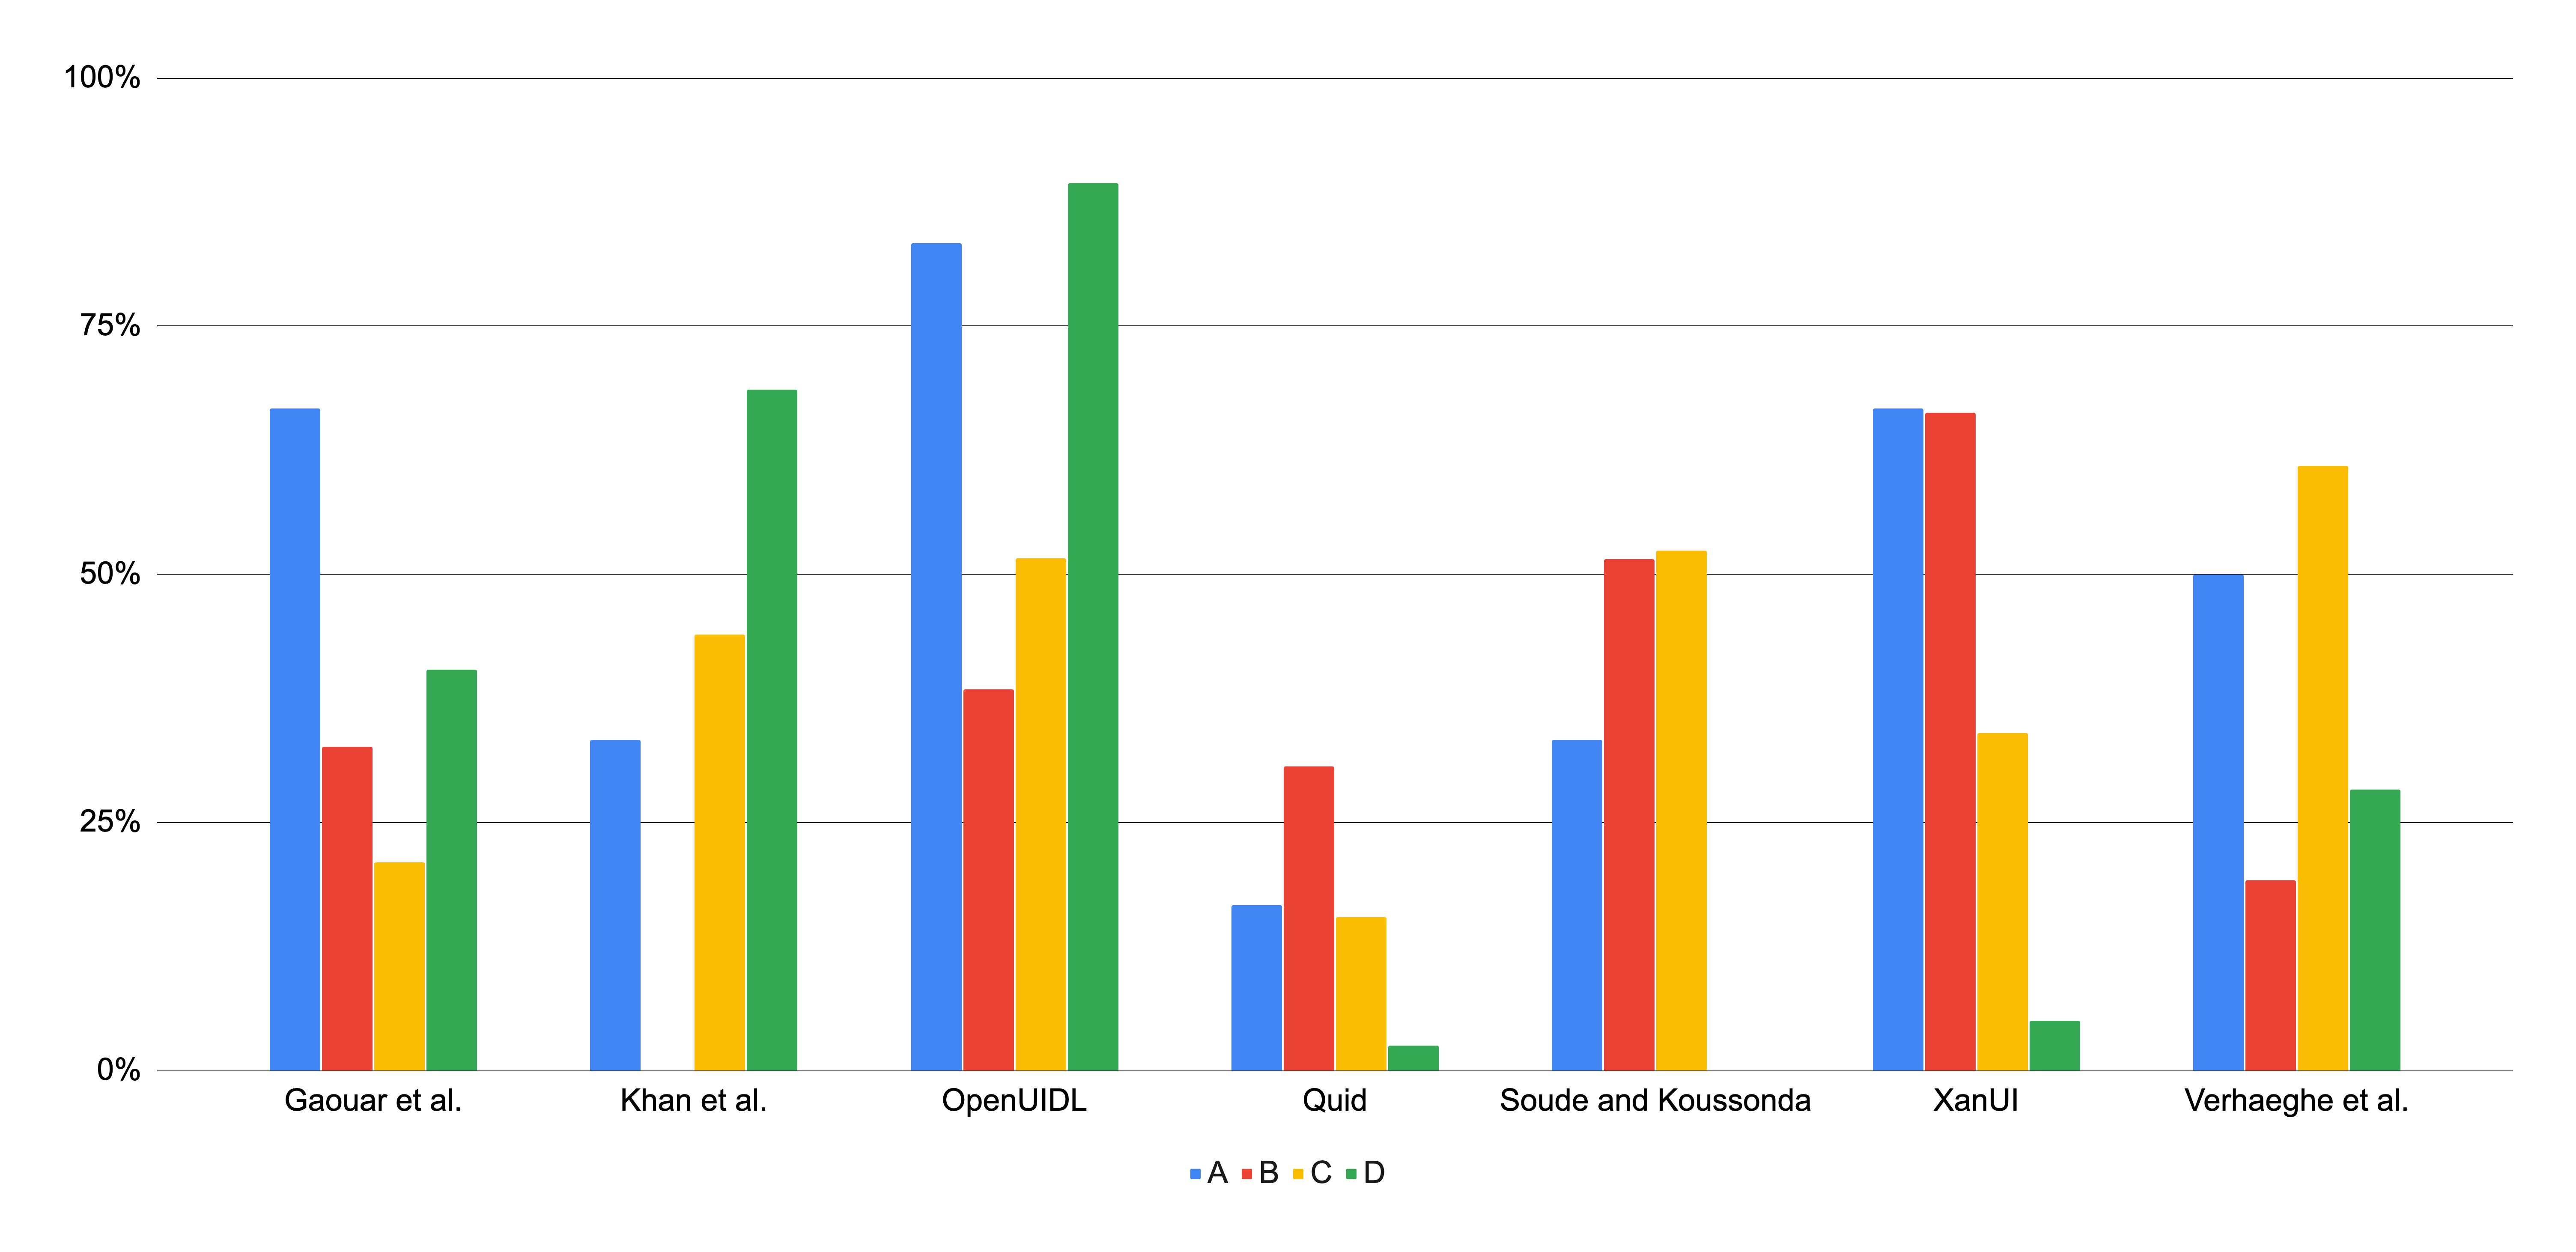
\includegraphics[width=\textwidth]{4-results-and-discussion/results-per-representation}
    \caption{Results of the evaluation, presented per representation}
    \label{fig:4-1-results-per-representation}
\end{figure}

\begin{figure}
    \centering
    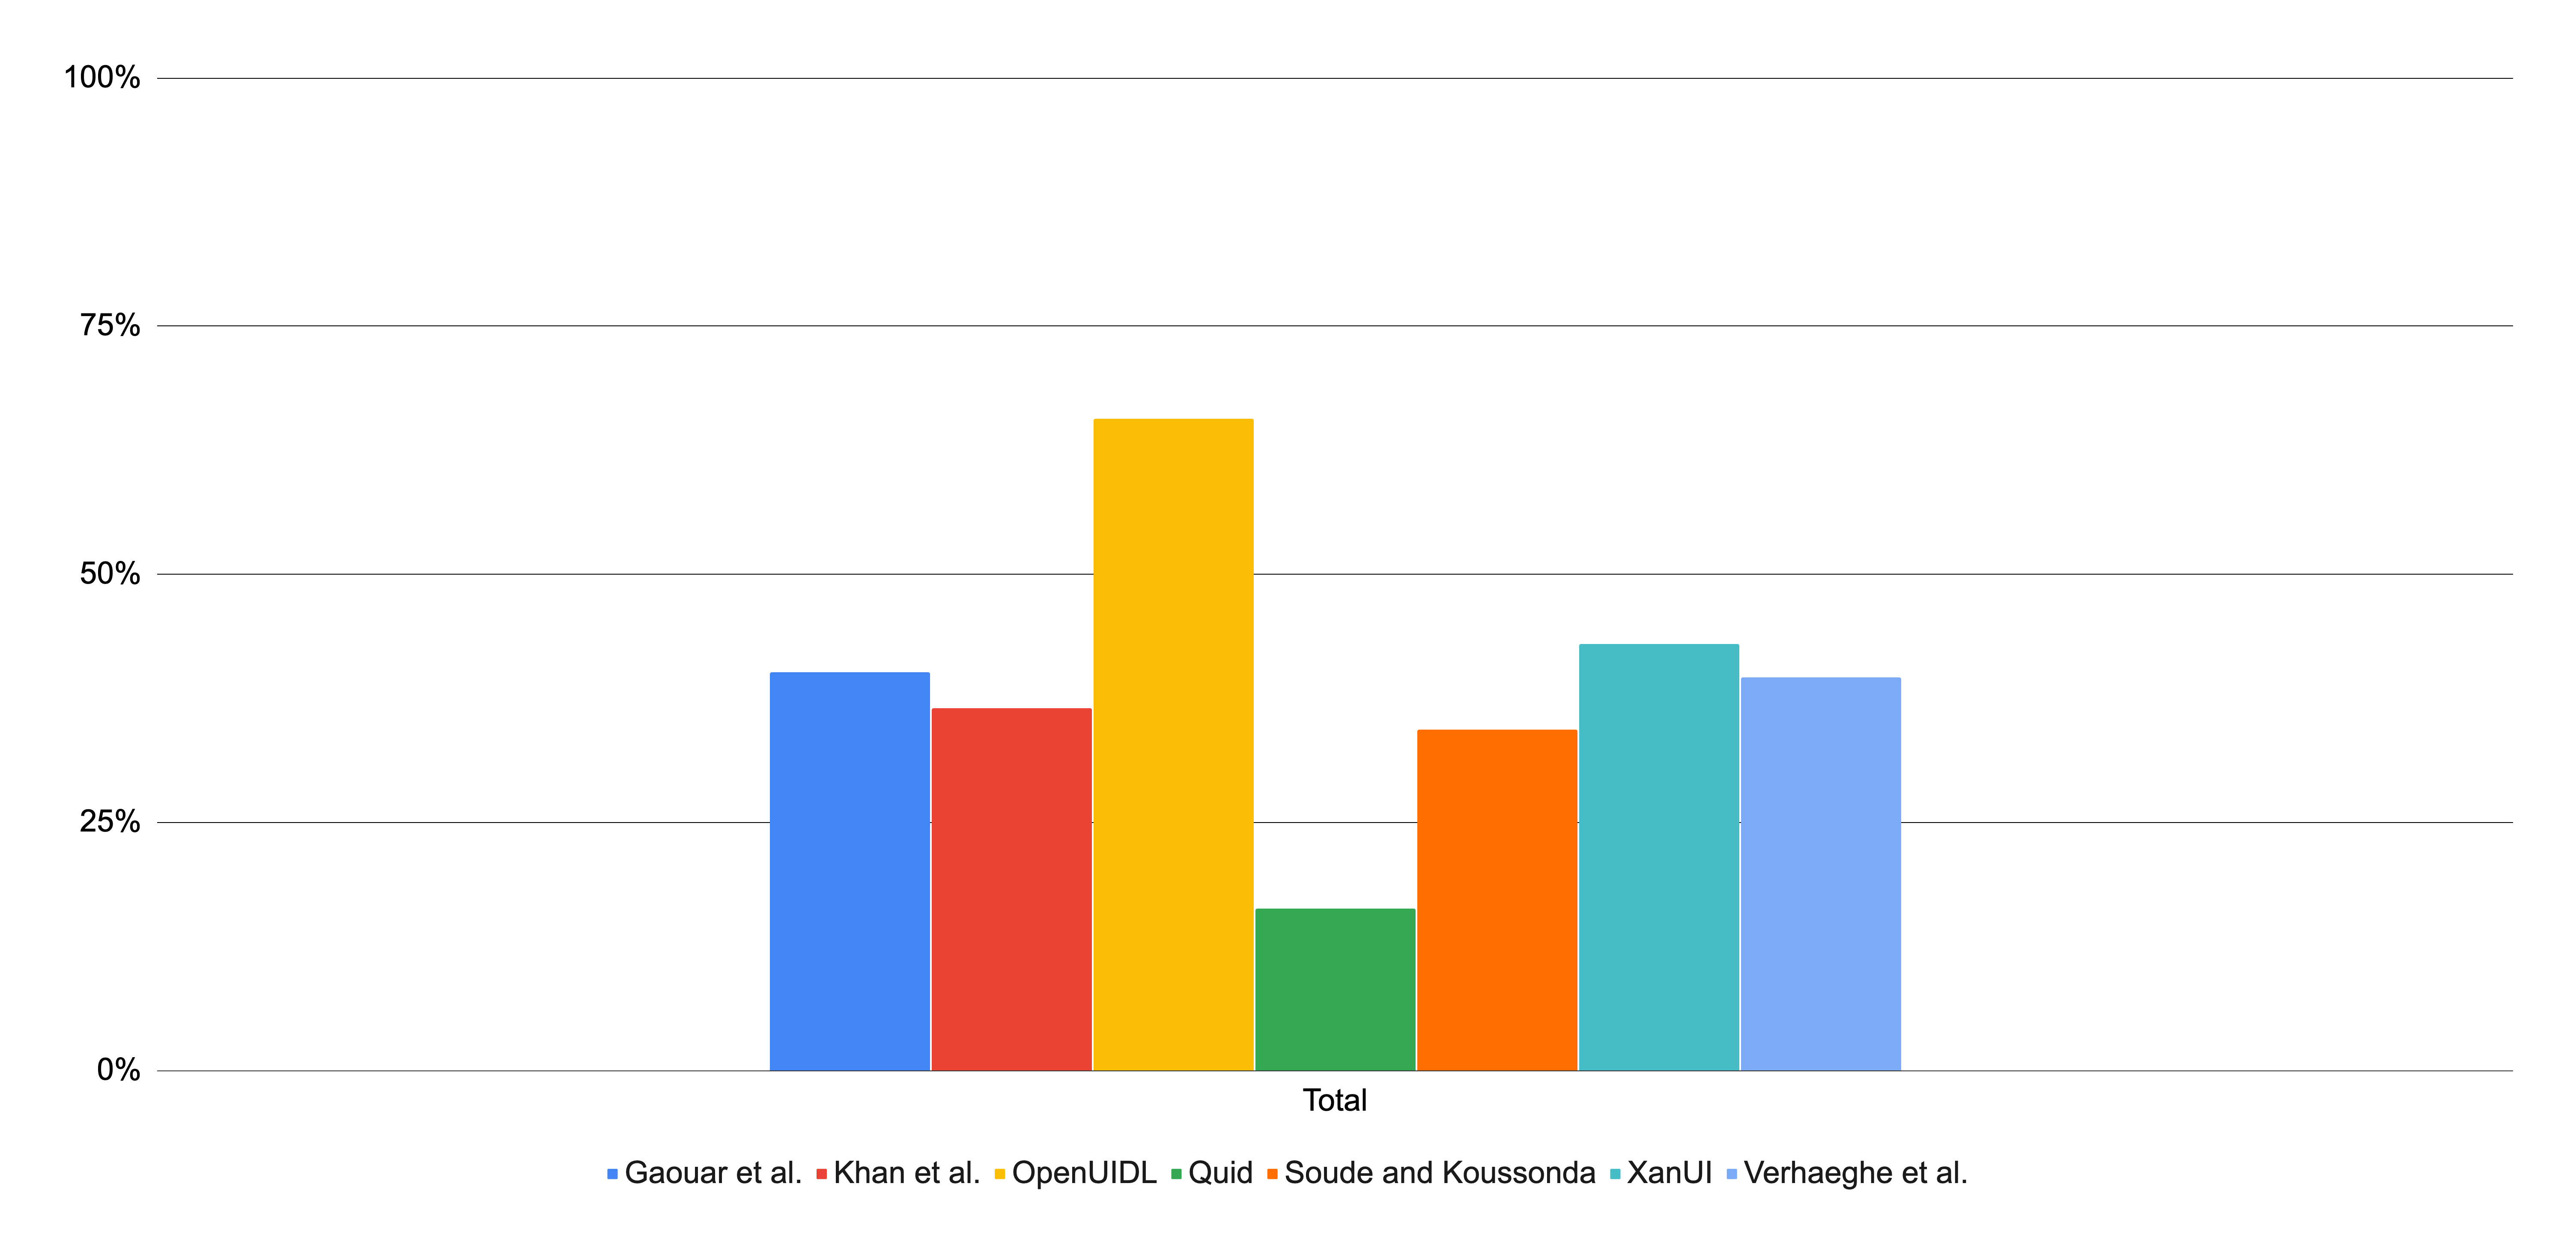
\includegraphics[width=\textwidth]{4-results-and-discussion/results-total}
    \caption{Overall results of the evaluation}
    \label{fig:4-1-results-total}
\end{figure}

\subsection{Results of the case study}\label{subsec:results-of-the-case-study}

The table~\ref{tab:4-1-case-study-results} presents the results of implementation of the application from the case study.
\begin{itemize}
    \item main takeaway: the results are very similar to the theoretical criteria!
    \item Quid isn't very expressive \textendash\ it's barely possible to do anything
    \item OpenUIDL actually allows to do something \textendash\  it was possible to prototype and customize quite a bit; the only thing missing was state and logic management (even though some was already present in a very primitive form!)
\end{itemize}
Figure~\ref{fig:4-1-board-view} presents the board view, as implemented in the selected languages.

\begin{longtblr}[
    caption = {Results of the case study},
    label = {tab:4-1-case-study-results},
]{
    colspec = {ccccccc},
    rowhead = 1,
    rows = {m},
}
    \hline[1pt]
    \textbf{Req. no.} & \textbf{Quid} & \textbf{OpenUIDL} & & \textbf{Req. no.} & \textbf{Quid} & \textbf{OpenUIDL} \\*
    \hline[1pt]
    \textbf{Total}    & 13,48\%       & 69,26\%           & & \textbf{R4}       & 0,00\%        & 64,29\%           \\*
    \cline{1-3}
    \textbf{R1}       & 12,50\%       & 62,50\%           & & R4.1              & 0             & 1                 \\*
    R1.1              & 0             & 1                 & & R4.2              & 0             & 1                 \\*
    R1.2              & 0             & 0                 & & R4.3              & 0             & 0,5               \\*
    R1.3              & 0,5           & 0,5               & & R4.4              & 0             & 0                 \\*
    R1.4              & 0             & 1                 & & R4.5              & 0             & 0                 \\*
    \cline{1-3}
    \textbf{R2}       & 33,33\%       & 66,67\%           & & R4.6              & 0             & 1                 \\*
    R2.1              & 0             & 0                 & & R4.7              & 0             & 1                 \\*
    \cline{5-7}
    R2.2              & 1             & 1                 & & \textbf{R5}       & 9,09\%        & 59,09\%           \\*
    R2.3              & 0             & 1                 & & R5.1              & 0             & 1                 \\*
    \cline{1-3}
    \textbf{R3}       & 12,50\%       & 93,75\%           & & R5.2              & 0             & 1                 \\*
    R3.1              & 0             & 1                 & & R5.3              & 0             & 0                 \\*
    R3.2              & 0             & 1                 & & R5.4              & 0             & 1                 \\*
    R3.3              & 0,5           & 1                 & & R5.5              & 1             & 1                 \\*
    R3.4              & 0             & 1                 & & R5.6              & 0             & 1                 \\*
    R3.5              & 0,5           & 1                 & & R5.7              & 0             & 0,5               \\*
    R3.6              & 0             & 1                 & & R5.8              & 0             & 1                 \\*
    R3.7              & 0             & 1                 & & R5.9              & 0             & 0                 \\*
    R3.8              & 0             & 0,5               & & R5.10             & 0             & 0                 \\*
                      &               &                   & & R5.11             & 0             & 0                 \\*
    \hline[1pt]
\end{longtblr}

\begin{figure}
    \centering
    \begin{subfigure}[m]{0.6\textwidth}
        \centering
        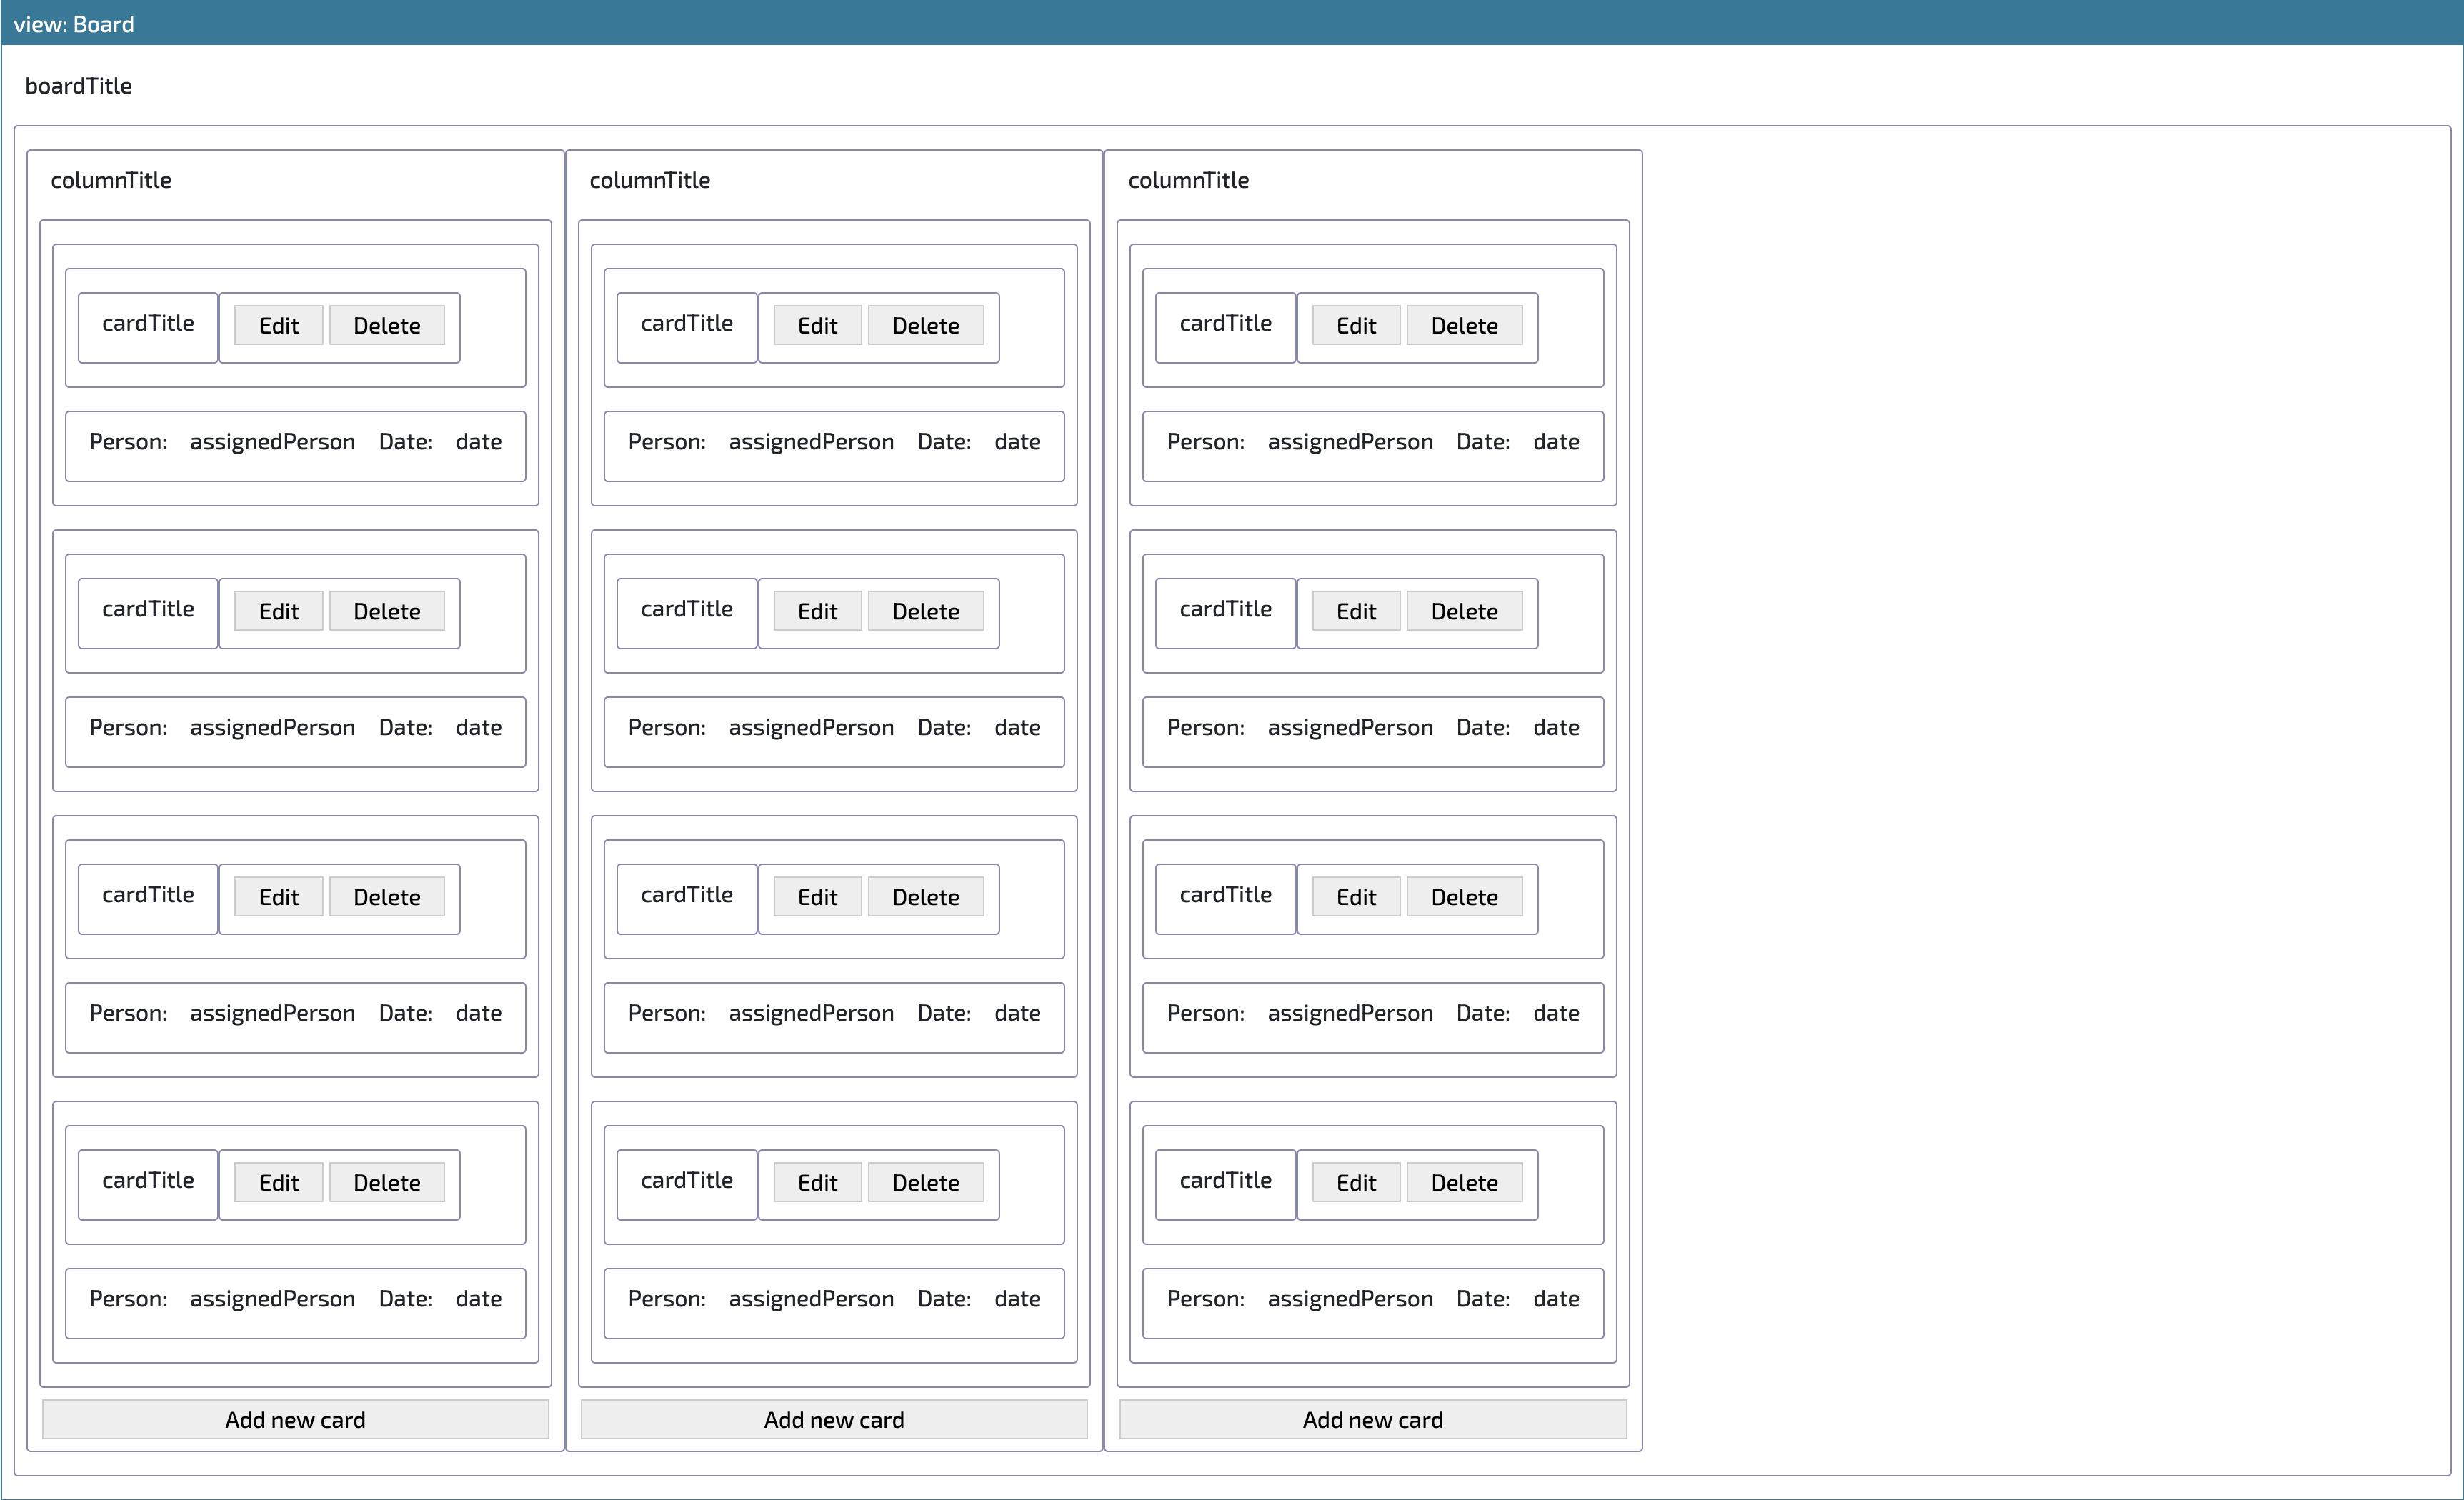
\includegraphics[height=0.25\textheight]{./4-results-and-discussion/quid-board-view}
        \caption{Board view implemented in Quid}
        \label{fig:4-1-quid-board-view}
    \end{subfigure}
    \hfill
    \begin{subfigure}[m]{0.35\textwidth}
        \centering
        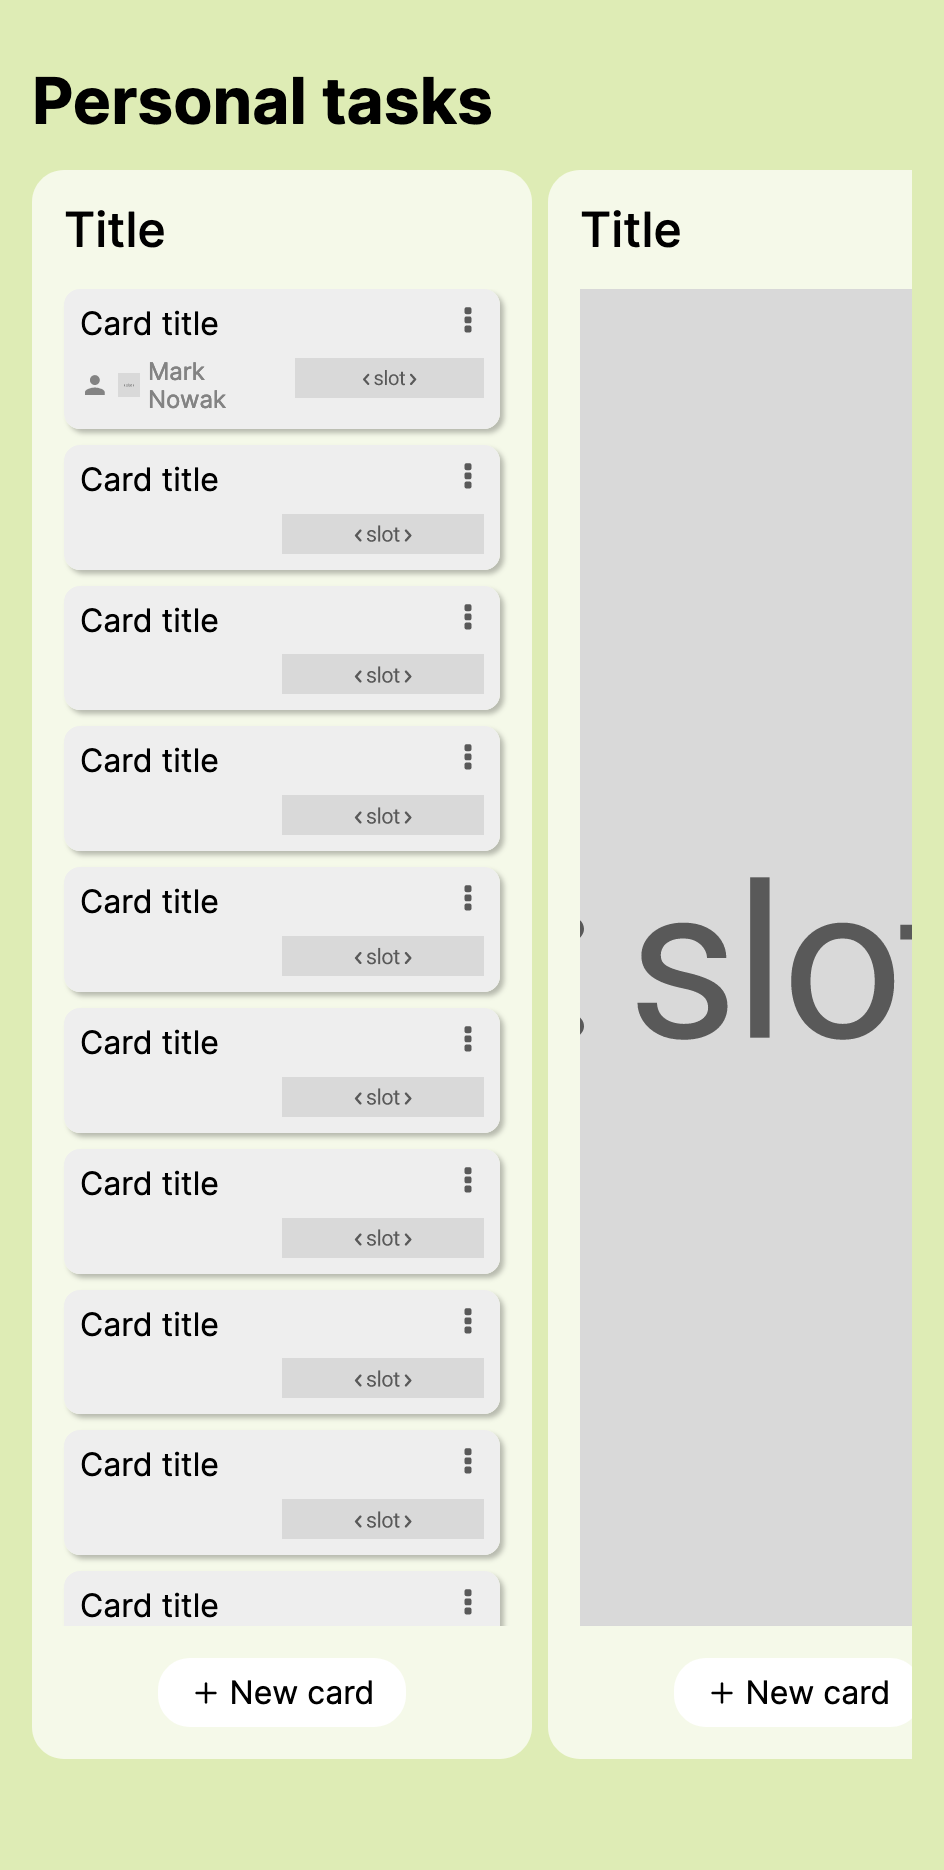
\includegraphics[height=0.4\textheight]{./4-results-and-discussion/openuidl-board-view}
        \caption{Board view implemented in OpenUIDL}
        \label{fig:4-1-openuidl-board-view}
    \end{subfigure}
    \caption{Implementations of the board view from the case study}
    \label{fig:4-1-board-view}
\end{figure}

\subsection{Results of the qualitative evaluation}\label{subsec:results-of-the-qualitative-evaluation}

Some initial thoughts:
Quid
\begin{itemize}
    \item the initial idea is great - the minimal language, the live preview
    \item the execution is lacking
    \item currently, the solution could be only viewed as a proof of concept, but nothing productive (not version 1.0 yet), the project doesn't seem maintained
    \item the documentation is too short and not detailed
\end{itemize}

OpenUIDL:
\begin{itemize}
    \item OpenUIDL looks like a relatively mature (and commercialized) solution, is well integrated with other solutions (deploying to some CDNs, integration with GitHub, etc.)
    \item there seems a lot of potential, but the capabilities for logic seem underdeveloped and can only be used to create simple, static pages
    \item the language is hidden behind an editor UI which is a good idea, because it could be difficult to write big projects
    \item in this way, though, it's impossible to use the language directly
    \item that the UI is a little buggy
\end{itemize}
